\documentclass{beamer}
\usepackage{colortbl}
\usepackage{etex}
\input{/home/mnattaf/Documents/input_latex/usepackage.tex}
\usepackage[T1]{fontenc}
\usepackage[utf8]{inputenc}
\usepackage[english]{babel}
\usepackage{pgfpages}
\usepackage{blindtext}
\usepackage{pgfplots}
\usepackage[lang=en]{templateLAAS}

\newtheorem{prop}{Proposition}
% \addtobeamertemplate{footline}{\insertframenumber/\inserttotalframenumber}

\setbeamersize{text margin left=25pt}
\setbeamersize{text margin right=25pt}
\input{/home/mnattaf/Documents/input_latex/newcommand.tex}


\title{Scheduling Under Energy Constraints}
\author{Margaux NATTAF}
\institute{LAAS-CNRS Toulouse

  Université Paul Sabatier Toulouse}


\setbeamertemplate{itemize item}[ball]
\setbeamertemplate{itemize subitem}[triangle]
\setbeamertemplate{itemize subsubitem}[circle]

\newcolumntype{M}[1]{>{\centering\arraybackslash}m{#1}}

\begin{document}

{\canvasspecial
  \begin{frame}
    \vspace{1.5cm}
    \begin{flushleft}
      {\Large \bf \color{bleuLAAS}SCHEDULING UNDER ENERGY CONSTRAINTS}
      
      \vspace{0.3cm}
      \small \color{bleuLAAS!90} defended by Margaux NATTAF

      October 18, 2016
    \end{flushleft}
    \vspace{0.5cm}

    {\footnotesize  \color{bleuLAAS!80}
      Supervised by Christian ARTIGUES \& Pierre LOPEZ}

    \vspace{1.5cm}
    \begin{flushright} \color{bleuLAAS!70}
      \scriptsize LAAS-CNRS, Toulouse

      Université Paul Sabatier, Toulouse
    \end{flushright}
  \end{frame}}

\setcounter{framenumber}{0}


\setcounter{tocdepth}{1}
\begin{frame}{Overview}
  \tableofcontents[hideothersubsections,subsubsectionstyle={show/show/show/show}]
\end{frame}

\section{Introduction}

\begin{frame}{What is {\it Scheduling}?}
  \vspace{0.3cm}
  \begin{block}{Definition {\small \it \color{blue!50!black!50}[Pinedo, 2008]}}
    Scheduling deals with the allocation of {\bf resources} to {\bf tasks} over
    given \textbf{time} periods and its goal is to optimize one or more \textbf{objectives}.
  \end{block}
\pause
  \vspace{0.3cm}
  {\bf Goal:} Decide when execute the tasks, i.e. when allocate resources
  to the tasks.
\pause
\vspace{0.3cm}

  Sometimes also how much resources give to the tasks.
  \vspace{0.5cm}
 {\small  \begin{description}[constraints :]
    \pause
  \item[tasks :]  courses, landing/taking off, step in project,
    production operation... 
    \pause
  \item[constraints :]
    \begin{itemize}
    \item temporal $\rightarrow$ deadline, precedence, setup...
    \item resource $\rightarrow$ availability, nature... 
    \end{itemize}
    \pause
  \item[objective :] resource consumption, total cost, makespan...
  \end{description}}
\vfill
\end{frame}


\begin{frame}
  \frametitle{The Cumulative Scheduling Problem} 
  \vspace{0.1cm}
  \textbf{Inputs : }
  \vspace{0.15cm}
  \begin{itemize}
  \item a set ${\cal A}=\{1,\dots ,n\}$ of {\bf non-preemptive} tasks
    \vspace{0.15cm}
  \item a {\bf cumulative} and {\bf renewable} resource available in quantity $B$
    \vspace{0.15cm}
  \item for each task:
    \vspace{-1cm}
    \begin{columns}
      \hfill
      \begin{column}{0.36\linewidth}
        \begin{itemize}
        \item \footnotesize  a processing time $p_i$
        \item \footnotesize a resource consumption $b_i$ 
        \item \footnotesize a release date $r_i$ and a deadline $d_i$ 
        \end{itemize}
      \end{column}
      \begin{column}{0.7\linewidth}
        \centering
        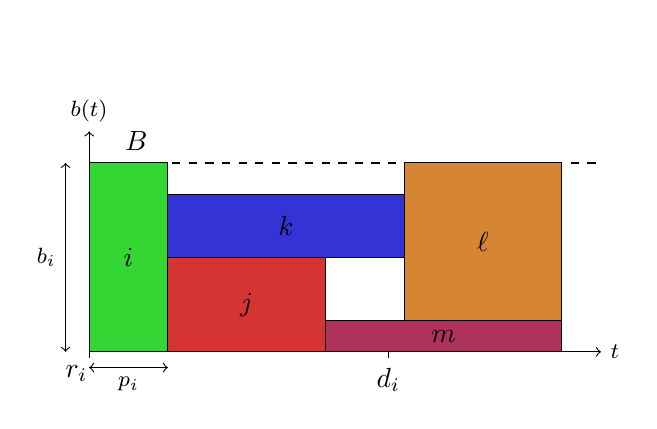
\begin{tikzpicture}
  [yscale=0.4]
  \node at (0,10) {};

  \node[label={[shift={(-0.4,-0.5)}]}] (O) at (0,0) {};
  \draw[fill=red!80!black!80] (1,0) rectangle (3,3)   node[midway] {$j$};
  \draw[dashed,thick] (0,6)   -- (6.5,6);
  \node at (0.6,6.7)  {$B$};
    \draw[<->] (0,-0.5) -- (1,-0.5) node[midway,below] {\footnotesize $p_i$};
    \draw[<->] (-0.3,0) -- (-0.3,6) node[midway,left] {\footnotesize $b_{i}$};
  
  \draw (0,0) -- (0,-0.2) node[below=0.2cm,left=-0.1cm] {$r_i$};
  \draw (3.8,0) -- (3.8,-0.2) node[below] {$d_i$};
  
  \draw[fill=green!80!black!80] (0,0) rectangle (1,6)   node[midway] {$i$};
  \draw[fill=blue!80!black!80] (1,3) rectangle (4,5)   node[midway] {$k$};
  \draw[fill=orange!80!black!80] (4,1) rectangle (6,6)   node[midway] {$\ell$};
  \draw[fill=purple!80!black!80] (3,0) rectangle (6,1)   node[midway] {$m$};
  \draw[->] (O.center) -- (0,7) node[above] {\footnotesize $b(t)$};
  \draw[->] (O.center) -- (6.5,0) node[right] {\footnotesize $t$};


\end{tikzpicture}

      \end{column} 
    \end{columns}
  \end{itemize}
  \vspace{-0.5cm}
  \textbf{Application : }
  \vfill
  \begin{itemize}
  \item electricity consumption cannot exceed a certain level.
  \end{itemize}
\end{frame}

\begin{frame}{Continuous/Discrete resource} 
  \begin{description}
  \item[Continuous resource:] ~
  \end{description}
  
  \vspace{-0.3cm}
  \begin{itemize}
  \item {\small non-integer \textcolor{blue!80!black!80}{allocation}}

    {\footnotesize $\rightarrow$ task $i$ consumes \textcolor{blue!80!black!80}{$\mathbf{3.5}$} units of resource}
  \item {\small non-integer \textcolor{red!80!black!80}{time } }
    
    {\footnotesize $\rightarrow$ task $i$ consumes $3$ units of resource in \textcolor{red!80!black!80}{$\mathbf{[1.5,2]}$}}
  \end{itemize} 

  \vspace{0.2cm} 
  \begin{description}
  \item[  Discrete resource:] ~
  \end{description}

  \vspace{-0.3cm}
  \begin{itemize}
  \item {\small integer \textcolor{blue!80!black!80}{allocation }}

    {\footnotesize $\rightarrow$ task $i$ consumes \textcolor{blue!80!black!80}{$\mathbf{3}$} units of resource}
  \item {\small integer \textcolor{red!80!black!80}{time }}

    {\footnotesize $\rightarrow$ task $i$ consumes $3$ units of resource in \textcolor{red!80!black!80}{$\mathbf{[1,2]}$}}
  \end{itemize}

  \vspace{0.2cm} 
  \begin{center}
    {\footnotesize
      \begin{tabular}{|c|c|c|}
        \hline
        & Continuous Time & Discrete Time\\
        \hline
        Continuous allocation & \cellcolor{blue!80!black!80}&   \cellcolor{blue!50!black!20}\\
        \hline
        Discrete allocation & &  \cellcolor{blue!50!black!20}\\
        \hline
      \end{tabular}}
  \end{center}
\end{frame}


\begin{frame}
  \frametitle{Limitations of the CuSP}
  \vspace{0.5cm}
  \begin{itemize}
  \item {Limitation} : tasks have fixed duration and resource consumption
    \vfill
  \item<2-> But, in practice, it is not always the case\\
  \end{itemize}
  \vspace{0.6cm}
  \begin{columns}
    \hfill
    \begin{column}{0.45\linewidth}
      \centering
      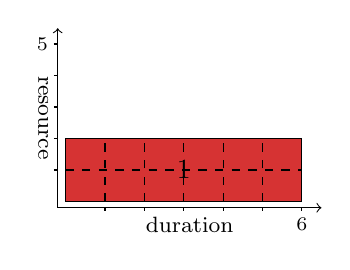
\begin{tikzpicture}
        [xscale=0.5,yscale=0.4]
        \node (O) at (0,0) {};
        \draw[fill=red!80!black!80] (0,0) rectangle (6,2) node[midway] {$1$};
        \draw[->](-0.2,-0.2) -- (-0.2,5.5)
        node[midway,below,rotate=-90] {\footnotesize resource};
        
        
        \draw[->] (-0.2,-0.2) -- (6.5,-0.2) node[midway,below]
        {\footnotesize duration};
        \foreach \i in {1,...,5}{
          \draw (-0.3,\i) -- (-0.2,\i);
          \draw (\i, -0.3) -- (\i,-0.2);
        }
        \onslide<3->{
          \draw (-0.3,5) -- (-0.2,5) node[left] {\scriptsize  $5$};
          \draw (6, -0.3) -- (6,-0.2) node[below] {\scriptsize  $6$};
          \draw[dashed] (0,0) grid (6,2);
        }
      \end{tikzpicture}
    \end{column}
    \hfill
    \begin{column}{0.45\linewidth}
      \centering
      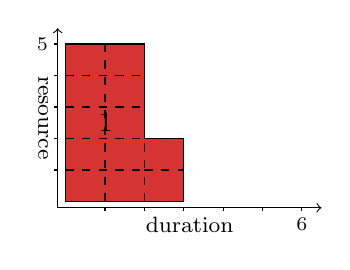
\begin{tikzpicture}
        [xscale=0.5,yscale=0.4]
        \node (O) at (0,0) {};
        \onslide<3->{
          
          \draw[->] (-0.2,-0.2) -- (6.5,-0.2) node[midway,below] {\footnotesize duration};

          \path[draw,fill=red!80!black!80] (0,0) node[above=1cm,right=0.3cm] {$1$}-- (0,5) -- (2,5) -- (2,2) -- (3,2) -- (3,0)-- cycle;
          \draw[->](-0.2,-0.2) -- (-0.2,5.5)
          node[midway,below,rotate=-90] {\footnotesize resource};
          \foreach \i in {1,...,5}{
            \draw (-0.3,\i) -- (-0.2,\i);
            \draw (\i, -0.3) -- (\i,-0.2);}

          \draw (-0.3,5) -- (-0.2,5) node[left] {\scriptsize $5$};
          \draw (6, -0.3) -- (6,-0.2) node[below] {\scriptsize  $6$};
          \draw[dashed] (0,0) grid (2,5);
          \draw[dashed] (2,0) grid (3,2);}
      \end{tikzpicture}
    \end{column}
    \hfill
  \end{columns}

  \vspace{0.3cm}
  \onslide<4->{
    A required {\bf energy} quantity ({\bf [resource $\times$ time]}, e.g. MW/h , pers./day) is associated to a task.
  }
\end{frame}


% \begin{frame}{Motivating Problem
%   {\small \it \color{gray!50!black!50} [Artigues et al., 2013]}} 
%   \vfill
%   \begin{block}{}
%     \begin{center}


%       \vspace{0.2cm}
%       \includegraphics[scale=0.1]{pipe.jpg}

%       \begin{tikzpicture}[yscale=.6]
%         \node (O) at (0,0) {};
%         \draw[-latex,ultra thick, bleuLAAS!100!black!50] (O.center) -- (-3,-1.5);
%         \draw[-latex,ultra thick, bleuLAAS!100!black!50] (O.center) -- (0,-1.5);
%         \draw[-latex,ultra thick, bleuLAAS!100!black!50] (O.center) -- (3,-1.5);

%         \node[draw] at (-3.4,-2.1) {drawing mill}; 
%         \node[draw] at (3.5,-2.1) {pipe-tubing};

%         \node[draw] at (0,-2.1) {\textbf<4>{foundry}};
%       \end{tikzpicture}
%     \end{center}
%   \end{block}
%   \vfill
%   \pause
%   \begin{itemize}
%   \item melting and heating use a {\bf HUGE} quantity of energy
%     \vfill
%     \pause
%   \item $\Rightarrow$ high electricity cost:
%     \begin{itemize}
%     \item total energy consumed
%     \item penalty for power overrun
%     \end{itemize}
%   \end{itemize}
% \end{frame}

\begin{frame}
  \frametitle{Motivating Problem 
    {\small \it \color{gray!50!black!50} [Artigues et al., 2013]}}
  \vfill 
  \begin{block}{\bf \large  pipe-manufacturing plant} 
    melting and heating use a {\bf HUGE} quantity of energy
  \end{block}
  \vfill
  \begin{columns}
    \begin{column}{0.5\linewidth}
      \begin{itemize}
      \item a set of melting jobs
        \vspace{0.4cm}
      \item melting operation has variable duration\\
        {\small (depending of the power given + may vary over time)}
        \vspace{0.4cm}
      \end{itemize}     
    \end{column}
    \hfill 
    \begin{column}{0.4\linewidth}
      \onslide<1->{  \includegraphics[width=0.8\linewidth]{figures/induction.jpg}}
    \end{column}
  \end{columns}
  \vfill
  \begin{itemize}
  \item upper and lower bound on the instantaneous power given \\
    {\small(operational and physical consideration)}
    \vspace{0.4cm}
  \item electrical power limitation\\
    {\small(electrical overrun cost)}
  \end{itemize}
\end{frame}

\begin{frame}
  \frametitle{Literature review}
  \begin{itemize}
    \vfill
  \item {\bf Cumulative Scheduling Problem (CuSP)},
    {\color{gray!50!black!50} \it [Erschler \& Lopez, 1990] }, {\color{blue!80!black!80} fixed resource consumption}
    \vfill
    \pause
  \item {\bf Fully elastic scheduling}, {\color{gray!50!black!50} \it [Baptiste et al., 1999]}, {\color{blue!80!black!80} no upper and lower bound on the consumption}
    \vfill
    \pause
  \item {\bf Variable Intensity}, {\color{gray!50!black!50} \it [Kis, 2005]}, {\color{blue!80!black!80} no lower bound on the consumption}
    \vfill  
    \pause
  \item {\bf Scheduling with continuous resource}, {\color{gray!50!black!50}\it [Blazewicz et al., 2006]}, {\color{blue!80!black!80}  no upper and lower bound}
    \vfill
    \pause
  \item {\bf Multimode activities}, {\color{gray!50!black!50}\it [De Reyck
      et al., 1998]},
    {\color{blue!80!black!80} tasks have rectangular shape}
  \end{itemize}
  \vfill
\end{frame}


\begin{frame}{The CECSP : definition }
  Generalization of the CuSP
  \begin{itemize}
    \vfill
  \item duration $p_i$ $\leftrightarrow$ required energy  $W_i$
    \vfill
  \item fixed resource consumption $b_i$ $\leftrightarrow$ variable
    resource consumption $b_i(t)$ 
    \vfill  
  \item Task can take any shape bounded by:
    \begin{itemize}
    \item its \textcolor<1>{blue!80!black!80!}{time-window}
    \item a \textcolor<1>{green!60!black!80}{maximal and minimal resource consumption}
    \item \textcolor<1>{red!80!black!80}{energy amount} that has to be received by the task
    \end{itemize}
    \vfill
  \end{itemize}
  \begin{overlayarea}{\textwidth}{3cm}
    \only<1> {
      \vfill
      \begin{columns}
        \begin{column}{0.45\linewidth}
          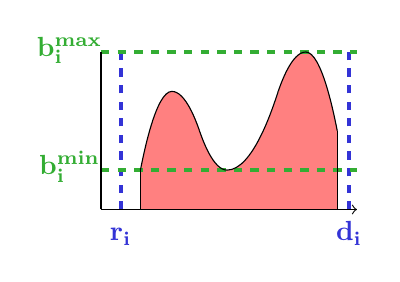
\begin{tikzpicture}
  [scale=0.5]
  \node (O) at (0,0) {};
  \fill[red!50] (1,0) -- (1,1) parabola bend (1.8,3)(2.51,2) -- (2.51,0);
  \fill[red!50] (2.49,0) -- (2.5,2) parabola bend (3.2,1) (4.511,3) -- (4.511,0) ;
  \fill[red!50] (4.489,0) -- (4.5,3) parabola bend (5.2,4) (6,2) -- (6,0);

  \node[label={[shift={(0,-0.7)}]\color{blue!80!black!80}$\mathbf{r_i}$}]  at (0.5,0) {};
  \node[label={[shift={(0,-0.7)}]\color{blue!80!black!80}$\mathbf{d_i}$}]  at (6.3,0) {};
  \draw[ultra thick,dashed,color=blue!80!black!80] (0.5,0) -- (0.5,4);
  \draw[ultra thick,dashed,color=blue!80!black!80] (6.3,0) -- (6.3,4);
  
    \node[label={[shift={(-0.4,-0.4)}]\color{green!60!black!80}$\mathbf{b_i^{min}}$}]  at (0,1) {};
    \node[label={[shift={(-0.4,-0.4)}]\color{green!60!black!80}$\mathbf{b_i^{max}}$}]  at (0,4) {};
    \draw[ultra thick,dashed,color=green!60!black!80] (0,1) -- (6.5,1);
    \draw[ultra thick,dashed,color=green!60!black!80] (0,4) -- (6.5,4);
  
  \draw (O.center) -- (0,4);
  \draw[->] (O.center) -- (6.5,0);
  
  \draw (1,1) -- (1,0);
  
  
  \draw (1,1) parabola bend (1.8,3)(2.5,2); 
  \draw (2.5,2) parabola bend (3.2,1) (4.5,3);
  \draw (4.5,3) parabola bend (5.2,4) (6,2);
  
  \draw (6,2) -- (6,0);
\end{tikzpicture}

        \end{column}
        \begin{column}{0.45\linewidth}
          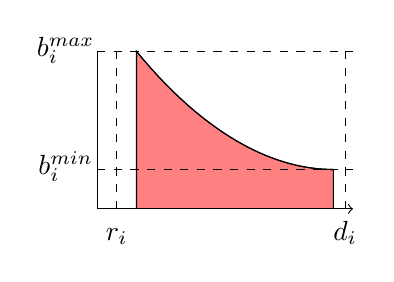
\begin{tikzpicture}
  [scale=0.5]
  \node (O) at (0,0) {};
  \onslide<4->{  
    \path[draw, fill=red!50] (1,0) -- (1,4) parabola [bend at end] (6,1) -- (6,0); 
  }
  \onslide<2->{
    \node[label={[shift={(0,-0.7)}]$r_i$}]  at (0.5,0) {};
    \node[label={[shift={(0,-0.7)}]$d_i$}]  at (6.3,0) {};
    \draw[dashed] (0.5,0) -- (0.5,4);
    \draw[dashed] (6.3,0) -- (6.3,4);
  }
  \onslide<3->{
    \node[label={[shift={(-0.4,-0.4)}]$b_i^{min}$}]  at (0,1) {};
    \node[label={[shift={(-0.4,-0.4)}]$b_i^{max}$}]  at (0,4) {};
    \draw[dashed] (0,1) -- (6.5,1);
    \draw[dashed] (0,4) -- (6.5,4);}
  
  
  \draw (O.center) -- (0,4);
  \draw[->] (O.center) -- (6.5,0);
  
  \draw (1,4) -- (1,0);
  
  
  \path[draw] (1,4) parabola [bend at end] (6,1); 
  
  \draw (6,1) -- (6,0);
\end{tikzpicture}

        \end{column}
      \end{columns}
      \vfill}
    \only<2>{
      \vfill
      \begin{itemize}
      \item Modeled with a continuous resource
      \end{itemize}
      \vfill 
      $\Rightarrow$ \textbf{Continuous Energy-Constrained Scheduling Problem (CECSP) {\scriptsize \color{gray!50!black!50} \it [Artigues \& Lopez, JoS, 2015]}}
      \vfill}
  \end{overlayarea}
\end{frame}

\begin{frame}
  \frametitle{Problem statement}
  \vfill
  Input:\\
  \begin{itemize}
  \item $A=\{1,\hdots,n\}$ a set of non-preemptive tasks
  \item a {\bf continuous}, {\bf cumulative} and {\bf renewable} resource of capacity  $B$
  \end{itemize}
  \vfill
  \onslide<2->{
    Output: A scheduling, i.e. a start time $st_i$, an end time $et_i$ and a resource allocation function $b_i(t)$, such that:
  }
  \begin{overlayarea}{\linewidth}{1cm}
    \only<3>{\[{\color{red!80!black!80}r_i}\le st_i\le et_i \le {\color{red!80!black!80}d_i}\]}
    \only<4>{\[{\color{red!80!black!80}\bmin} \le b_i(t) \le {\color{red!80!black!80}\bmax} \quad \forall t \in \inter[st_i][et_i]\]}
    \only<5>{\[b_i(t)={\color{red!80!black!80}0}\quad \forall t \not\in \inter[st_i][et_i]\]}
    \only<6>{\[\int_{st_i}^{et_i}b_i(t)dt=W_i\]}
    \only<7>{\[\sum_{i\in A}b_i(t) \le {\color{red!80!black!80}B}\]} 
  \end{overlayarea}
  \onslide<2->{
    \begin{center}
      \input{figures/form2_bi.tex}
    \end{center}}
\end{frame}

\begin{frame}
  \frametitle{Example}
  \begin{center}
    \begin{tabular}{cccccc}
      \hline
      $i$ & $r_i$ & $d_i$ & $W_i$ & $b_i^{min}$ & $b_i^{max}$ \\
      \hline
      {\color<2->{red!80!black!80}$1$} &
                                          {\color<2->{red!80!black!80}$0$} & {\color<2->{red!80!black!80}$6$} & {\color<2->{red!80!black!80} $12$} & {\color<2->{red!80!black!80} $1$ }& {\color<2->{red!80!black!80} $5$} \\
      $2$ & $2$ & $6$ & $12$ & $2$ & $5$ \\
      $3$ & $2$ & $5$ & $6$ & $2$ & $2$ \\
      \hline
    \end{tabular}
  \end{center}
  
  \begin{columns}
    \begin{column}{0.45\linewidth}
      \onslide<1->{
        \begin{tikzpicture}
[scale=0.7]
\node (O) at (0,0) {};
\node[label={[shift={(-0.4,0)}]$B=5$}] (B) at (0,5) {};

\onslide<3->{
\node[label={[shift={(-0.4,-0.4)}]\color{red!80!black!80}$b_1^{min}$}] (B) at (0,1) {};
\node[label={[shift={(-0.4,-0.4)}]\color{red!80!black!80}$b_1^{max}$}] (B) at (0,5) {};
}

\node (r1) at (0,-0.5) {{\color<3->{red!80!black!80}$est_1$}}; 
\node (r2) at (2,-0.5) {$est_2$};
\node (r3) at (2,-0.9) {$est_3$};
\node (d1) at (6,-0.5) {{\color<3->{red!80!black!80}$let_1$}};
\node (d2) at (6,-0.9) {$let_2$};
\node (d3) at (5,-0.5) {$let_3$};


\draw[->,>=latex] (6,0) -- (6.5,0);

%\draw (0,0) rectangle (6,5);
\draw[fill=blue!80!black!80] (4,0) -- (6,0) -- (6,5) -- (5,5) -- (5,3) -- (2,3) -- (2,1) --
(4,1) --cycle;
\onslide<2-3>
    {\draw[fill=red!80!black!80] (2,5) -- (2,1) -- (4,1) -- (4,0) -- (0,0) -- (0,5) -- cycle;}
\onslide<3->
    {\draw[fill=red!80!black!80] (2,5) -- (2,1) -- (4,1) -- (4,0) -- (0,0) -- (0,5) -- cycle;}
% \onslide<7>
%     {\draw[fill=red!80!black!80] (2,5) -- (2,0) -- (0,0) -- (0,5)-- cycle;
%       \draw[fill=red!80!black!80,pattern=north west lines, pattern color=red!80!black!80] (2,1) -- (4,1) -- (4,0)-- (2,0) -- cycle;
%     }
% \onslide<8->
%     {\draw[fill=red!80!black!80,pattern=north west lines, pattern color=red!80!black!80] (2,1) -- (4,1) -- (4,0)-- (0,0) --(0,5)--(2,5) -- cycle;
%     }
\draw[fill=orange!80!black!80]  (2,3) -- (5,3) -- (5,5) -- (2,5) --cycle;


\node (2) at (4,2) {\LARGE $2$};
\node (1) at (1,2) {\LARGE $1$};
\node (3) at (3.5,4) {\LARGE $3$};
\foreach \i in {0,...,5}
{
  \draw (\i,-0.3) -- (\i,0);
  \draw (-0.3,\i) -- (0,\i);
}

 \draw (6,-0.3) -- (6,0);

\end{tikzpicture}

      }
    \end{column}
    \hfill
    \begin{column}{0.45\linewidth}
      \newbox\hautbox \setbox\hautbox=\hbox{\vphantom{\rule[-0.4cm]{0cm}{0.9cm}}}
      \begin{tabular}{@{\usebox{\hautbox}}l}
        \onslide<3->{$\int_0^{4} b_1(t)dt=?$} \\
        \onslide<4->{$\int_0^{2}${\color<4>{red!80!black!80}{$5$}}$dt +\int_2^{4}${\color<4>{red!80!black!80}{$1$}}$dt$\\
        $=10+2=12$}
      \end{tabular}
    \end{column}
    \hfill
  \end{columns}
\end{frame}


\begin{frame}{The CECSP : limitations}
  \vfill
  \begin{itemize}
  \item Consider that the resource consumed by the task is proportional to
    the energy received by the task.
    \vfill
    \pause
  \item Not always the case...
  \end{itemize}
  \vfill
  \pause
  \begin{block}{Example of the foundry}
    Give twice more power to the furnace $\not\Rightarrow$ Task
    finishes twice faster... 
  \end{block}
  \vfill

\end{frame}

  % \begin{block}{Example in parallel architecture}
  %   \begin{itemize}
  %   \item a set of tasks has to be scheduled on parallel processors;
  %     \pause
  %   \item resource : processors;
  %     \pause
  %   \item energy : elementary operation;
  %     \pause
  %   \item Typical power speed function:  $b^{\alpha} , \ 0 <
  %     \alpha \le 1$ (may be different for each task)
  %     \pause
  %   \end{itemize}
  % \end{block}


\begin{frame}{The CECSP : limitations}
  \begin{itemize}
  \item   $\Rightarrow$ We need to model {\bf conversion functions} $f_i$.
    \vfill
    \pause
  \item  We have considered the case where $f_i(b)$ is non-decreasing,
    continuous and  
    \pause
    \begin{enumerate}
      \vspace{0.5cm}
    \item linear: $f_i(b)=a_i*b+c_i(1-\delta_{b0})$ 

      \vspace{0.1cm}
      $\rightarrow$ the {\bf CECSP$_{lin}$}
      \vspace{0.5cm}
      \pause
    \item concave and piecewise linear: if $f$ has $P$ pieces,
      $f_i(b)=a_{ip}*b+c_{ip}(1-\delta_{b0}) , p \in \{1,\dots,P\}$

      \vspace{0.1cm}
      $\rightarrow$ {\bf the CECSP$_{cpwl}$} 
    \end{enumerate}
    \vfill
    \pause
  \item   \[W_i=\int_{st_i}^{et_i}b_i(t)dt \rightarrow
      W_i=\int_{st_i}^{et_i}{\color{red!80!black!80}\mathbf{f_i}(}b_i(t)
      {\color{red!80!black!80})}dt\]   
    \vfill
    \pause
  \item   linear and concave piecewise linear approximation of more
    general efficiency functions.
  \end{itemize}
  \vfill
\end{frame}

\begin{frame}
  \frametitle{Concave Efficiency Function}
  $f_i$ are continuous, non-decreasing and {\bf concave} efficiency functions 
  \vfill
  \begin{columns}
    \begin{column}{0.45\linewidth}
      \begin{figure}
        \centering
        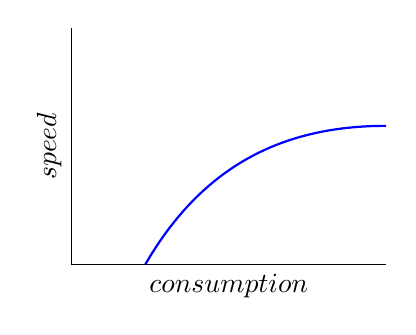
\begin{tikzpicture}
          \node (O) at (0,0) {};
          \draw (0,0) -- (4,0) node[midway,below] {$consumption$};
          \draw (0,0) -- (0,3) node[midway,left] {\rotatebox{90}{$speed$}};
          \draw[thick,blue] (0.94,0) to [bend left] (4,1.76);
        \end{tikzpicture}
        \caption{Speed vs. fuel consumption\footnotemark}
      \end{figure}
    \end{column}
    \hfill
    \begin{column}{0.45\linewidth}      
      \vspace{0.2cm}
      \begin{figure}
        \centering    
        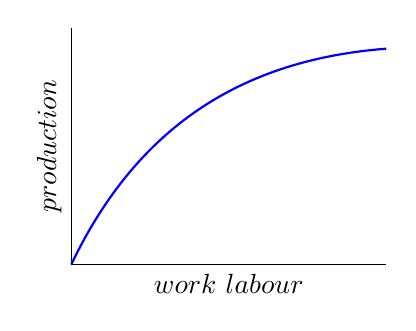
\begin{tikzpicture}
          \node (O) at (0,0) {};
          \draw (0,0) -- (4,0) node[midway,below] {$work\ labour$};
          \draw (0,0) -- (0,3) node[midway,left] {\rotatebox{90}{$production$}};
          \draw[thick,blue] (0,0) to [bend left] (4,2.74);
        \end{tikzpicture}      
        \caption[\footnotesize]{ Work Labour vs. production rate\footnotemark}
      \end{figure}
    \end{column}
    \hfill
  \end{columns}
  \footnotetext[1]{\tiny Algebra Symposium: Optimizing Fuel Consumption}
  \footnotetext[2]{\tiny Non-convex agreggative technology
    and optimal economic growth}
\end{frame}


\begin{frame}{Approximation by below of efficiency functions}
  \vfill
  \begin{columns}
    \begin{column}{0.5\linewidth}
      \begin{figure}[!htb]
\captionsetup{justification=centering}
        \centering
        \begin{tikzpicture}
          [xscale=0.55,yscale=0.35]
          \node (O) at (0,0) {};
          
          \draw[dotted] (7,0) node[below] {$\bmax$} -- (7,7);
          \draw[dotted] (1,0) node[below] {$\bmin$} -- (1,7);
          \draw[->] (O.center) -- (8,0) node [below] {$b$};
          \draw[->] (O.center) -- (0,7) node [left] {$f(b)$};
          \draw[gray!80] (0,0.01) parabola bend (0.5,0.01) (3.6,3.4);
          \draw[gray!80] (3.6,3.4) parabola bend (6.5,6) (7.5,6);

          \draw[densely dashed] (1.25,0) -- (7,6);
        \end{tikzpicture}
        \caption{Approximation by a linear function}
      \end{figure}
    \end{column}
    \pause
    \begin{column}{0.5\linewidth}
      \begin{figure}[!htb]
        \centering
\captionsetup{justification=centering}
        \begin{tikzpicture}
          [xscale=0.55,yscale=0.35]
          \node (O) at (0,0) {};
          
          \draw[dotted] (7,0) node[below] {$\bmax$} -- (7,7);
          \draw[dotted] (1,0) node[below] {$\bmin$} -- (1,7);
          \draw[->] (O.center) -- (8,0) node [below] {$b$};
          \draw[->] (O.center) -- (0,7) node [left] {$f(b)$};
          \draw[gray!80] (0,0.01) parabola bend (0.5,0.01) (3.6,3.4);
          \draw[gray!80] (3.6,3.4) parabola bend (6.5,6) (7.5,6);

          \draw[densely dashed]  (6,5.9) -- (7,6);
          \draw[densely dashed]  (6,5.9) -- (5,5.3);
          \draw[densely dashed] (4,4.05) -- (5,5.3);
          \draw[densely dashed]  (3,2.1) -- (4,4.05);
          \draw[densely dashed] (1.5,0) -- (3,2.1);
        \end{tikzpicture}
        \caption{Approximation by a concave piecewise linear function}
      \end{figure}
    \end{column}
  \end{columns}

\end{frame}

\begin{frame}{Example for the CECSP$_{lin}$}
  

\begin{columns}
  \begin{column}{0.5\linewidth}
    \begin{center}
      {\small \begin{tabular}{|M{0.4cm}|M{0.4cm}M{0.4cm}M{0.4cm}M{0.4cm}M{0.4cm}M{1.2cm}|}
        \hline
        $i$ & $r_i$ & $d_i$ & $W_i$ & $\bmin$ & $\bmax$ & $f_i(b)$\\[1mm]
        \hline
        1 & 0 & 2 & 6 & 3 & 3 & $b$\\[1mm]
        \color<3->{red!80!black!80}2 & \color<3->{red!80!black!80}1 & \color<3->{red!80!black!80}5 & \color<3->{red!80!black!80}22 & \color<3->{red!80!black!80}3 & \color<3->{red!80!black!80}4 & \color<3->{red!80!black!80}$\rightarrow$ \\[1mm]
         3 & 0 &6 & 45 & 1 & 5 & $3b+1$\\[1mm]
        \hline
        \multicolumn{7}{c}{}
      \end{tabular}}
    \end{center}
  \end{column}
\hfill
    \begin{column}{0.4\linewidth}
\begin{tikzpicture}
[xscale=0.8,yscale=0.45]
\node (O) at (2,5) {};
\draw[->] (2,4) -- (5.5,4) node[below] {$b$}; 
\draw[dashed] (2,4) -- (2,5.5);
\draw[->] (2,5.5) -- (2,10) node[left] {$f_2(b)$};


\path[draw] (3,6) -- (4,8) -- (5,9) ;

\draw[dotted] (3,4) node[below] {\footnotesize $3$} -- (3,10);
\draw[dotted,color=gray!70] (4,4) node[below,color=black] {\footnotesize $4$}
-- (4,10);
\draw[dotted] (5,4) node[below] {\footnotesize $5$} -- (5,10);

\draw (2,6) node[left] {\footnotesize $6$};
\draw (2,8) node[left] {\footnotesize $8$};
\draw (2,9) node[left] {\footnotesize $9$};
\end{tikzpicture}
\end{column}
\end{columns}
\pause
  \begin{columns}
    \begin{column}{0.45\linewidth}
      \onslide<2->{
        \centering
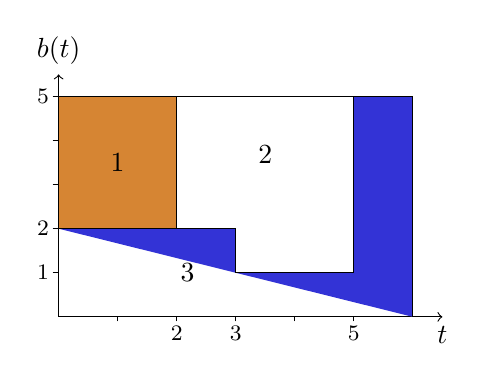
\begin{tikzpicture}
[xscale=0.75,yscale=0.56]
\node (O) at (0,0) {};
\draw[->] (0,0) -- (6.5,0) node[below] {$t$};
\draw[->] (0,0) -- (0,5.5) node[above] {$b(t)$};

\draw[fill=orange!80!black!80] (0,2) rectangle (2,5) node[midway] {$1$};
\path[draw,fill=blue!80!black!80] (0,2) -- (3,2) -- (3,1) node[left=0.4cm] {$3$} -- (5,1) -- (5,5) -- (6,5)  -- (6,0);
\draw[fill=red!80!black!80] (2,5) -- (5,5) node[midway,below=0.5cm] {$2$};

\draw (0,1) node[left] {\footnotesize $1$};
\draw (0,2) node[left] {\footnotesize $2$};
\draw (0,5) node[left] {\footnotesize $5$};


\draw (2,0) node[below] {\footnotesize $2$};
\draw (3,0) node[below] {\footnotesize $3$};
\draw (5,0) node[below] {\footnotesize $5$};

\foreach \i in {1,...,5}{
\draw (\i,-0.1) -- (\i,0);
\draw (-0.1,\i) -- (0,\i);
}
\end{tikzpicture}

      }
    \end{column}
    \hfill
       \begin{column}{0.45\linewidth}{
\vspace{-0.1cm}       
       \small
      \newbox\hautbox \setbox\hautbox\hbox{\vphantom{\rule[-0.4cm]{0cm}{0.8cm}}}
      \begin{tabular}{@{\usebox{\hautbox}}l}
        \onslide<4->{$\int_2^{5} f_2(b_2(t))dt=?$} \\
        \onslide<5->{$\int_2^{3} f_2(3) dt$}\onslide<6->{$+\int_3^{5} f_2(4) dt$=}\\
	    \onslide<7->{$\int_2^{3} 6 dt$}\onslide<8->{$+\int_3^{5} 8 dt$=}\\
       \onslide<9->{$6$}\onslide<10->{$+16=$}\onslide<11->{$22$}\onslide<12->{$\
        \neq
        \int_2^5 b_2(t)dt = 11 $}\\
              \end{tabular}}
    \end{column}
    \hfill
  \end{columns}

\end{frame}


\begin{frame}
  \frametitle{Problem statement}
  \vfill
 {\small  {\bf Input: } 
  \begin{itemize}
  \item $A=\{1,\hdots,n\}$ a set of non-preemptive tasks
  \item a continuous, cumulative and renewable resource of capacity  $B$
  \end{itemize}
  \vspace{0.5cm}
  {\bf Output:} a start/end time $st_i/et_i$ and a res. allocation function
  $b_i(t)$ s.t.:
  {\footnotesize
    \begin{align}
    r_i\le st_i\le
   et_i \le d_i & & \tag{{\it \scriptsize
                                                     time-window}}\\
    \bmin \le b_i(t) \le \bmax & & \forall t
                                                                 \in \inter[st_i][et_i] \tag{{\it \scriptsize min/max consump.}}\\
    b_i(t)=0 & &
                                               \forall t \not\in \inter[st_i][et_i] \tag{{\it \scriptsize no
                                               consump.}}\\ 
    \int_{st_i}^{et_i}f_i(b_i(t))dt=W_i
                                                 & &\tag{{\it \scriptsize energy}} \\
    \sum_{i\in A}b_i(t) \le B & & \tag{{\it
                                                                \scriptsize cumulative}}
  \end{align}
}

  \vspace{0.5cm}
{\bf Possible objective:} $\qquad $ minimize  $\sum_{i\in A}
\int_{st_i}^{et_i} b_i(t)dt $}
\end{frame}

\begin{frame}
  \frametitle{Solution methods}
  \vfill
  \begin{description}[Properties]
  \item[Properties] {\small
      \begin{itemize}
      \item study of the structural properties of the problem:
        {\footnotesize Dominance rules, complexity analysis, polynomial cases...}
      \end{itemize}}
    \vfill
    \pause
  \item[CP] {\small
      \begin{itemize}
      \item satisfiability test (checker): {\footnotesize Energetic
          reasoning, Flow based checker...}
      \item filtering algorithm: {\footnotesize Energetic reasoning, time-table
          disjunctive reasoning...}
      \item discrete model
      \end{itemize}}
    \vfill
    \pause
  \item[MILP] {\small
      \begin{itemize}
      \item MILP model: {\footnotesize time-indexed, event-based...}
      \item valid inequalities
      \item polyhedral results
      \end{itemize}}
    \vfill
    \pause
  \item[Hybrid] {\small
      \begin{itemize}
      \item ``CP-like branching'' + MILP 
      \item valid inequalities deduced from ER
      \end{itemize}}
  \end{description}
\end{frame}


\setcounter{tocdepth}{2}
\AtBeginSection[]
{
  \begin{frame}
    \frametitle{Overview}
    \thispagestyle{empty}  
    \tableofcontents[sectionstyle=show/shaded,subsectionstyle=show/show/hide
    ] 
  \end{frame}
  \addtocounter{framenumber}{-1}
}
\section{Problem Properties}

\begin{frame}
  \frametitle{Helpful remarks}
  scheduling a task at $\bmax$ during $\inter$ gives the higher energy amount ($f_i$ is non decreasing)
  \begin{center}
    \begin{tikzpicture}
      [yscale=0.6]
      [inner sep=0]
      \node (O) at (0,0) {};
      \node (T) [right of=O,node distance=4cm] {};
      \node (t1) [right of =O, node distance=1cm] {};
      \node (t2) [right of =t1, node distance=2cm] {};
      \draw[pattern=north west lines] (t1) rectangle (3,2.5);
      \draw[dashed,gray!40!] (0,2.5) -- (4,2.5) node[right] {$\bmax$};
      
      \draw[red,dashed] (t1) node[below] {$t_1$}-- (1,3);
      \draw[red,dashed] (t2) node[below] {$t_2$} -- (3,3);
      \draw[->] (O) -- (T);
    \end{tikzpicture}
  \end{center}
  
  \begin{block}{Notations}
    \begin{itemize}
    \item the latest start time of $i$ as $\smax=d_i-\frac{W_i}{f_i(\bmax)}$
    \item and the earliest end time of $i$ as $\emin=r_i+\frac{W_i}{f_i(\bmax)}$
    \end{itemize}
  \end{block}
  $\Rightarrow$ a task can start in $\inter[r_i][\smax]$ and end in $\inter[\emin][d_i]$
\end{frame}

\begin{frame}
  \frametitle{Trick for the MILP formulation}
  \textbf{Question:} How formulate a continuous problem with a MILP?
  
  \begin{theorem}
    Any solution can be transformed in a solution where $\forall i \in A,\ b_i(t)$ is piecewise constant. 
  \end{theorem}
  \begin{proof}[Proof (Sketch)]
    \begin{columns}
      \begin{column}{0.55\linewidth}
        \begin{overlayarea}{\textwidth}{5cm}
          \only<1-8>{            
            \begin{itemize}
            \item<3-> $(t_q)$: series of start and end times
              \vspace{0.2cm}
            \item<4-> in $\inter[t_q][t_{q+1}]$, $b'_i(t)$ is set to the mean value of $b_i(t)$ over this interval
              \vspace{0.4cm}
            \item<8-> same resource and energy amount
              \vspace{0.4cm}
            \end{itemize}
            
          }
          \only<9>{
            \vspace{1cm}
            \centering 
            {\bf Remark: }we have only to \\
            change at $st_i$ or $ft_i$ \\
            \vspace{0.5cm}
            = ``events''
          }
        \end{overlayarea}
      \end{column}
      \begin{column}{0.45\linewidth}
        \onslide<2->{
          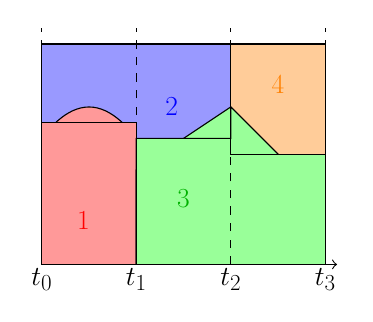
\begin{tikzpicture}
            [scale=0.4,transform shape]
            [inner sep =0]
            \node (O) at (0,0) {};
            \node (T) [right of=O,node distance=9.5cm] {};
            
            \fill[blue!40!,draw=black] (0,3) rectangle (6,7) node[midway, right=0.8cm] {\color{blue} \Huge $2$};
            \onslide<2-4>{
              \fill[red!40!,draw=black] (0,0) node[above right=1cm] {\color{red} \Huge$1$}-- (0,4) parabola bend (1.5,5) (3,4) --(3,0) -- cycle;}
            \onslide<5->{
              \fill[red!40!,draw=black] (0,0) node[above right=1cm] {\color{red} \Huge$1$}-- (0,4.5) --(3,4.5) --(3,0) -- cycle;}
            \fill[orange!40!,draw=black] (9,7) rectangle (6,2) node[midway, above= 0.8cm] {\color{orange} \Huge $4$};
            \onslide<2-5>{
              \fill[green!40!,draw=black] (3,0) -- (9,0) -- (9,2) -- (6,5)-- (3,3)  node[below, right=2cm] {\color{black!30!green} \Huge $3$}-- cycle;}
            \onslide<6>{
              \fill[green!40!,draw=black] (3,0) -- (9,0) -- (9,2) -- (6,5)-- (6,4)  node[left=1.5cm,below=1.5cm] {\color{black!30!green} \Huge $3$} --(3,4) -- cycle;
            };
            \onslide<7->{
              \fill[green!40!,draw=black] (3,0) -- (9,0) -- (9,3.5) -- (6,3.5)-- (6,4)  node[left=1.5cm,below=1.5cm] {\color{black!30!green} \Huge $3$} --(3,4) -- cycle;
            };
            \draw[->] (O) -- (T);
            \onslide<3->{
              \draw[dashed] (0,0) node[below] {\Huge $t_0$} -- (0,7.5);
              \draw[dashed] (3,0) node[below] {\Huge $t_1$} -- (3,7.5);
              \draw[dashed] (6,0) node[below] {\Huge $t_2$} -- (6,7.5);
              \draw[dashed] (9,0) node[below] {\Huge $t_3$} -- (9,7.5);
            }
          \end{tikzpicture}
        }
      \end{column}
    \end{columns}
\vspace{-1cm}
  \end{proof}
\end{frame}




\section{Mixed Integer Linear Progamming}

\begin{frame}
  \frametitle{Context}
  \begin{itemize}
  \item Time-indexed model more efficient {\small (relatively stronger relaxation)}
    \pause
    \vfill
  \item But:
    \begin{itemize}
    \item  model size depends on planning horizon 
      
      $\longrightarrow $ for large planning horizon event-based model can be more
      efficient (RCPSP:~{\color{gray!50!black!70}\it [Koné et al.,
        2011]} )
      \vfill
      \pause
    \item  if only non-integer solutions
      
      $\longrightarrow$ time-indexed model can lead to
      infeasible/sub-optimal solution
      (CECSP:~{\color{gray!50!black!70}\it [Nattaf et al., 2015]} )
    \end{itemize}
  \end{itemize}
  \vfill
  \pause
  {\bf Goal: Tightened Event-based models (2 exists)} 
\end{frame}
\begin{frame}{Start/End formulation}
  {\small \it Adaptation of a model for the RCPSP {\color{gray!50!black!50} \it [Koné et al., 2011]}}
  \vfill
  \begin{block}{Variables}
    \begin{itemize}
    \item  $t_e$ represents the event (start or end time)
      \pause
      \vspace{0.3cm}
    \item $x_{ie}=\left\{
        \begin{array}{ll}
          1 & \text{if $i$ starts at event $e$ (time $t_e$)}\\
          0 & \text{otherwise}
        \end{array}
      \right.
      $
      \pause
      \vspace{0.3cm}
    \item $y_{ie}=\left\{
        \begin{array}{ll}
          1 & \text{if $i$ ends at event $e$ (time $t_e$)}\\
          0 & \text{otherwise}
        \end{array}
      \right.
      $
      \vspace{0.3cm}
      \pause
    \item $B_{ie}$: resource quantity consumed by $i$ in $\inter[t_e][t_{e+1}]$
      \vspace{0.3cm}
      \pause
    \item $W_{ie}$: energy brought to $i$ in $\inter[t_e][t_{e+1}]$   
    \end{itemize}
  \end{block}
\end{frame}


\begin{frame}{Event-based model}
  \vfill
  \begin{itemize}
  \item Start/End model have stronger relaxations than the On/Off
    model ( $z_{ie} = \sum_{f=1}^e x_{if} - \sum_{f=1}^e y_{if}$)
    \pause
    \vfill
  \item But: On/Off model has less variables than Start/End model
    \pause
    and  better performances  
    \vfill
    \pause
  \item Study of the On-Off formulation
    \vfill
    \pause
  \item Collaboration with Tam{\'a}s Kis 
  \end{itemize} 
  \vfill
\end{frame}

\begin{frame}{Event-based model}
  \vfill 
  {\bf On/Off Model}
  {\footnotesize
    \begin{eqnarray*}
      \textcolor<1>{blue!80!black!80}{t_e \le t_{e+1} }&
                                                         \textcolor<1>{blue!80!black!80}{ \forall e}\\[2mm]
      \pause
      \textcolor<2>{blue!80!black!80}{r_iz_{ie}\le t_e
      } & \textcolor<2>{blue!80!black!80}{\forall e, i
          }\\[2mm] 
      \textcolor<2>{blue!80!black!80}{t_e \le
      lst_i(z_{ie}-z_{ie-1})+(1-(z_{ie}-z_{ie-1}))D_{max} }&
                                                             \textcolor<2>{blue!80!black!80}{ \forall e,i}\\[2mm]
      \pause
      \textcolor<3>{blue!80!black!80}{ 
      eet_i(z_{ie-1}-z_{ie})\le t_e} & \textcolor<3>{blue!80!black!80}{
                                       \forall e, i }\\[2mm]
      \textcolor<3>{blue!80!black!80}{t_e \le
      d_i(z_{ie-1}-z_{ie})+(1-(z_{ie-1}-z_{ie}))D_{max}}&
                                                            \textcolor<3>{blue!80!black!80}{\forall e, i }\\[2mm]
      \pause
      \textcolor<4>{blue!80!black!80}{ \sum_{e \in {\cal E}}
      z_{ie} \ge 1}& \textcolor<4>{blue!80!black!80}{\forall i
                     } \\[2mm]
      \textcolor<4>{blue!80!black!80}{\sum_{e'=1}^{e}
      z_{ie'} \le e(1-(z_{ie}-z_{ie-1})) }& \textcolor<4>{blue!80!black!80}{
                                            \forall e,i}\\[2mm]
      \textcolor<4>{blue!80!black!80}{\sum_{e'=e}^{2n}
      z_{ie'} \le (2n-e)(1+(z_{ie}-z_{ie-1})) }&
                                                 \textcolor<4>{blue!80!black!80}{\forall e,i}
    \end{eqnarray*}}
  \vfill
\end{frame}


\subsection{Valid inequalities}
\begin{frame}
  \frametitle{Maximum separation between events}
  \begin{itemize}
  \item {\bf Goal: } upper bound on the value of $t_{e+1}-t_{e}$
    \vspace{0.3cm}
  \item<2-> Time window of each task start and/or end time
    \vspace{0.3cm}
  \item<6-> An event must occur in each of these time windows
    \vspace{0.3cm}
  \item<11-> two consecutive events in the union of two consecutive time windows
  \end{itemize}
  \vfill
  \onslide<3->{
    \begin{center} 
      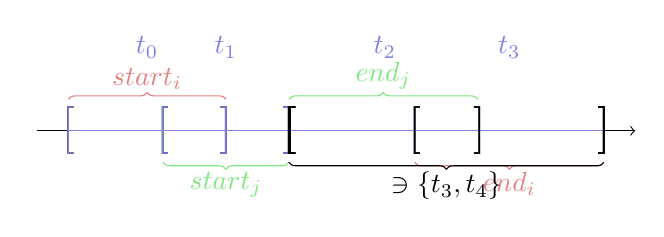
\begin{tikzpicture}
        [decoration={brace},scale=0.4]
        \node (O) at (0,0) {}; 
        \draw[->] (0,0) -- (19,0);

        \onslide<4-5>{
          \path (1,0) node[color=red!80!black!50] {\LARGE [} --
          +(0:5cm)node[color=red!80!black!50] {\LARGE ]};
          \path[green!80!black!50](4,0) node {\LARGE [} -- +(0:4cm)
          node {\LARGE ]};
          \path[green!80!black!50] (8.05,0) node {\LARGE [}  --
          +(0:6cm) node {\LARGE ]}  ;
          \path (12,0) node[color=red!80!black!50] {\LARGE [} --
          +(0:6cm) node[color=red!80!black!50] {\LARGE ]} ; 
        }
        
        \onslide<4>{
          \draw [decorate,color=red!80!black!50] (1,1) -- +(0:5cm)
          node[midway,above]{$start_i$}; 
          \draw [decorate,color=red!80!black!50] (18,-1) -- +(0:-6cm)
          node[midway,below] {$end_i$};
        }
        
        \onslide<5>{
          \draw [decorate,green!80!black!50] (8,-1) -- +(0:-4cm)
          node[midway,below] {$start_j$};
          \draw [decorate,green!80!black!50] (8,1) -- +(0:6cm)
          node[midway,above] {$end_j$};
        }
        
        \onslide<6-9>{
          \path (1,0) node {\LARGE [} --
          +(0:5cm)node {\LARGE ]};
          \path(4,0) node {\LARGE [} -- +(0:4cm)
          node {\LARGE ]};
          \path (8.05,0) node {\LARGE [}  --
          +(0:6cm) node {\LARGE ]}  ;
          \path (12,0) node {\LARGE [} --
          +(0:6cm) node {\LARGE ]} ; 
        }

        \onslide<6>{
          \path[blue!80!black!50,draw] (1,0) node {\LARGE [} -- +(0:5cm)node
          {\LARGE ]} node[midway,above=0.8cm] {$t_0$};
        }
        \onslide<7>  {
          \path[blue!80!black!50,draw](4,0) node {\LARGE [} --
          +(0:4cm) node {\LARGE ]} node[midway,above=0.8cm] {$t_1$}; 
        }
        
        \onslide<8>{   
          \path[blue!80!black!50,draw] (8.05,0) node {\LARGE [}  --
          +(0:6cm) node {\LARGE ]}  node[midway,above=0.8cm] {$t_2$};
        }
        
        \onslide<9>{
          \path[blue!80!black!50,draw] (12,0) node {\LARGE [} --
          +(0:6cm) node {\LARGE ]} node[midway,above=0.8cm] {$t_3$};
        }
        
        \onslide<10>{
          \path (12,0) node {\LARGE [}  --
          +(0:6cm) node {\LARGE ]}  ;
          \path (8.05,0) node {\LARGE [}  --
          +(0:6cm) node {\LARGE ]}  ;
        }
        \onslide<11>{
          \path (12,0) --
          +(0:6cm) node {\LARGE ]}  ;
          \path (8.05,0) node {\LARGE [}  --
          +(0:6cm)  ;
        }
        
        \onslide<12>{
          \path (8,0) node {\LARGE [} --
          +(0:10cm) node {\LARGE ]}  ;
          \draw [decorate] (18,-1) -- +(0:-10cm)
          node[midway,below] {$\ni \{t_3,t_{4}\}$};
        }
      \end{tikzpicture}
    \end{center}
  }
\end{frame}

\begin{frame}
  \frametitle{Maximum separation between events}
  \begin{itemize}
  \item Order the time-window intervals according to:
    \[ [a,b] \le [c,d]
      \Leftrightarrow a < c \lor \left( a=c \land b \le d\right)\]
    \vfill
    \pause
  \item Then we have:
    \[t_{e+1}-t_e  \le   |tw_e \cup tw_{e+1}|    \]
    \pause
    \begin{flushright}
      \textcolor{black!70}{\scriptsize in fact: $t_{e+1}-t_e  \le
        \overline{tw_e \cup tw_{e+1}} - \underline{tw_e \cup tw_{e+1}}
        $}
    \end{flushright}
    \pause
    \vfill
  \item We can use it as:
    \begin{itemize}
      \vspace{0.2cm}
    \item additional constraints of the model
    \item an upper bound on $t_{e+1}-t_e$ in any constraints using a worst one
    \end{itemize}
  \end{itemize}
\end{frame}

\begin{frame}
  \frametitle{Maximum time for an event}
  \begin{itemize}
  \item {\bf Goal: } upper bound on the value of $t_{e}$
    \vspace{0.4cm}
  \item<2-> upper bound of each task start and/or end time
    \vspace{0.4cm}
  \item<5-> an event must occur before each of these upper bounds
    \vspace{0.4cm}
  \end{itemize}
  \vfill
  \onslide<3->{
    \begin{center} 
      \begin{tikzpicture}
        [decoration={brace},scale=0.4]
        \node (O) at (0,0) {}; 
        
        \draw[->] (0,0) -- (19,0);
        \onslide<3>{
          \draw (1,0) node {\LARGE [} -- +(0:5cm)node {\LARGE ]}; 
          
          \draw(4,0) node {\LARGE [} -- +(0:4cm) node {\LARGE ]} ;
          
          \draw (8.05,0) node {\LARGE [}  --
          +(0:6cm) node {\LARGE ]}  ;
          \draw (12,0) node {\LARGE [} --
          +(0:6cm) node {\LARGE ]}  ;}
        \onslide<4>{
          
          \draw (1,0) node {} -- +(0:5cm)node {\LARGE ]}; 
          
          \draw(4,0) node {} -- +(0:4cm) node {\LARGE ]} ;
          
          \draw (8.05,0) node {}  --
          +(0:6cm) node {\LARGE ]}  ;
          \draw (12,0) node {} --
          +(0:6cm) node {\LARGE ]}  ;}
        \onslide<5>{
          \draw[color=blue!80!black!50] (0,0) node {} -- +(0:6cm)node {\LARGE ]}
          node[left,above=0.8cm] {$t_0$}; 
          \draw (8,0) node {\LARGE ]} ;
          \draw (8.05,0) node {}  -- +(0:6cm) node {\LARGE ]}  ;
          \draw (12,0) node {} -- +(0:6cm) node {\LARGE ]}  ;}
        
        \onslide<6>{
          \draw (6,0) node  {\LARGE ]}; 
          \draw[color=blue!80!black!50](0,0) -- (8,0) node {\LARGE ]} node[left,above=0.8cm] {$t_1$};
          \draw (8.05,0) node {}  --  +(0:6cm) node {\LARGE ]}  ;
          \draw (12,0) node {} --  +(0:6cm) node {\LARGE ]}  ;}
        
        \onslide<7>{
          \draw (6,0) node {\LARGE ]}; 
          \draw (8,0) node {\LARGE ]} ;
          \draw[color=blue!80!black!50] (0,0) node {}  -- (14,0) node {\LARGE ]} node[left,above=0.8cm] {$t_2$} ;
          \draw (18,0)node {\LARGE ]}  ;}
        
        \onslide<8>{
          \draw (6,0) node {\LARGE ]}; 
          \draw(8,0) node {\LARGE ]} ;
          \draw (14,0) node {\LARGE ]}  ;
          \draw[color=blue!80!black!50] (0,0) node {} -- (18,0) node {\LARGE ]}
          node[left,above=0.8cm] {$t_3$};} 
        
      \end{tikzpicture}
    \end{center}
  }
\end{frame}


\begin{frame}
  \frametitle{Maximum time for an event}
  \begin{itemize}
  \item Order the time-window interval upper bounds ${\cal UP}$ in
    increasing order 
    \vfill
    \pause
  \item Then we have:
    \[t_e \le  {\cal UP}_e\]
    \vfill
    \pause
  \item We can use it as:
    \begin{itemize}
      \vspace{0.2cm}
    \item additional constraints of the model
    \item an upper bound on $t_{e+1}-t_e$ in any constraints using a worst one
    \end{itemize}
  \end{itemize}
\end{frame}

\subsection{Polyhedral results}


\begin{frame}
  \frametitle{$Z_i$-polyhedron}
  \vspace{0.5cm}
  \onslide<1->{$\rightarrow$ Minimal set of inequalities defining the
    {\it ``$Z_i$-polyhedron''}.}
  \vspace{0.6cm}
  \onslide<2-> {  \begin{block}{$Z_i$-polyhedron}
      form of $z_i \in \{0,1\}^{|{\cal E}|}$ solution? \hspace{2.5cm}
      {\scriptsize (${\cal E}=$event set)}}
    \vspace{0.4cm}

    \onslide<4->{$\Rightarrow$ vector with consecutive-one property  and at least
      one $1$
      \begin{center}
        {\small e.g. $(0,0,1,1,1,0),\ (1,1,1,0,0,0),\ \dots$}
      \end{center}}
    \onslide<5->{     
      \[Z_i= conv\{z_i \in \{0,1\}^{|{\cal E}|} | z_i \text{ of the
          form } (0^*\, 1\, 1^*\, 0^*)\} \] }
    \vspace{-0.2cm}
  \end{block}
  \onslide<3->{\textcolor{black!70}{ \small\[z_{ie}=\left\{
          \begin{array}{ll}
            1 & \text{if task $i$ is in process between $t_e$ and $t_{e+1}$}\\
            0 & \text{otherwise}
          \end{array}
        \right.
      \]}}
\end{frame}

\begin{frame}
  \frametitle{Non-preemptive inequalities}

  \begin{itemize}
  \item $ z_{ie}-z_{if}+z_{ig} \le 1$ enforces
    $z_{if}$ to be $1$ for all $e<f<g$ s.t. $z_{ie}=z_{ig}=1$ 
  \end{itemize}
  \pause
  \vspace{0.4cm}
  \begin{block}{Non-preemptive inequalities }
    Generalization of constraints $ z_{ie}-z_{if}+z_{ig} \le 1$ to
    every subset of events of odd cardinality (GNP).
  \end{block}
  \pause
  \vspace{0.4cm}
  \[ZP_i=\{ z_i \in [0,1]^{\cal E} | z_i\text{ satisfies
      GNP inequalities and } \eqref{eq1}\}\] 
  \begin{equation}
    \text{ with }  \sum_{e \in \cal E} z_{ie} \ge 1 \quad \forall i \in \cal A  
    \label{eq1}  
  \end{equation}
  \pause
  \vspace{0.4cm}
  \begin{block}{Theorem}
    \[ZP_i=Z_i\]
  \end{block}
  \vspace{0.5cm}
\end{frame}


\begin{frame}
  \frametitle{Computational experience}
  \begin{itemize}
    \vfill
  \item Intel Core i7-4770 processor with 4 cores and 8Go of RAM
    \vfill
  \item OS: 64-bit Ubuntu 12.04
    \vfill
  \item MILP resolution: CPLEX 12.6 with 1 thread  
    \vfill
  \item Special separation procedure for non-preemptive cuts ($O(n^2)$)
    for node with depth less than 10
    \vfill
  \item time limit: 1000 seconds
    \vfill
  \end{itemize}
\end{frame}

\pgfplotstableread[row sep=\\,col sep=&]{
  tasks & Default & Int. & Time & Preem. & I+T+P \\
  20    & 164.14 & 182.2 & 167.3 & 330.9 & 154  \\
  25     & 635.4 & 727.3 & 629.5 & 822.4 & 389.9 \\
  30    & 968  & 851 & 961.4 & 914.8 & 813.8\\
}\mydata

\begin{frame}
  \frametitle{Time comparison for the CECSP}
  \begin{itemize}
  \item Instances of {\it [Nattaf et al.,2015]}
  \item 10 instances of 20, 25 and 30 tasks
  \end{itemize}

  \vspace{0.2cm}
  \begin{center}\begin{tikzpicture}
      \begin{axis}[ enlarge x limits=0.25,
        ybar,
        bar width=.4cm,  
        legend style={at={(0.5,1)},
          anchor=north,legend columns=-1},
        width=\textwidth,
        height=.6\textwidth,
        symbolic x coords={20,25,30},
        xtick=data,
        ymin=0,ymax=1100,
        ylabel={\small time (s)},
        xlabel={\small $\#tasks$}]
        \addplot table[x=tasks,y=Default]{\mydata};
        \addplot table[x=tasks,y=Int.]{\mydata};
        \addplot table[x=tasks,y=Time]{\mydata};
        \addplot table[x=tasks,y=Preem.]{\mydata};
        \addplot table[x=tasks,y=I+T+P]{\mydata};
        \legend{Default ,Int. , Time , Preem. ,I+T+P}
      \end{axis}
    \end{tikzpicture}
  \end{center}
\end{frame}

\pgfplotstableread[row sep=\\,col sep=&]{
  tasks & Default & Int. & Time & Preem. & I+T+P \\
  20    & 90.9 & 90.9 & 90.9 & 72.7 & 90.9\\
  25     &55.6 & 55.6 & 88.9 & 44.4 & 77.8\\
  30    & 10 & 20& 20& 10 &60\\
}\mydat
\begin{frame}
  \frametitle{Solved instances comparison for the CECSP}
  \begin{itemize}
  \item Instances of {\color{gray!50!black!70}\it [Nattaf et al., 2015]}
  \item 10 instances of 20, 25 and 30 tasks
  \end{itemize}

  \vspace{0.2cm}
  \begin{center}\begin{tikzpicture}
      \begin{axis}[ enlarge x limits=0.25,
        ybar,
        bar width=.4cm,  
        legend style={at={(0.5,1)},
          anchor=north,legend columns=-1},
        width=\textwidth,
        height=.6\textwidth,
        symbolic x coords={20,25,30},
        xtick=data,
        ymin=0,ymax=110,
        ylabel={\small $\%solved$},
        xlabel={\small $\#tasks$}]
        \addplot table[x=tasks,y=Default]{\mydat};
        \addplot table[x=tasks,y=Int.]{\mydat};
        \addplot table[x=tasks,y=Time]{\mydat};
        \addplot table[x=tasks,y=Preem.]{\mydat};
        \addplot table[x=tasks,y=I+T+P]{\mydat};
        \legend{Default ,Int. , Time , Preem. ,I+T+P}
      \end{axis}
    \end{tikzpicture}
  \end{center}
\end{frame}

\pgfplotstableread[row sep=\\,col sep=&]{
  tasks & Default & Int. &  Preem. & I+P \\
  30    & 34.8 & 30.3& 30.3& 33.1\\
}\mydat
  \begin{frame}
    \frametitle{Time comparison for the RCPSP}
    \begin{itemize}
    \item Instances of {\color{gray!50!black!70} \it [Koné et al., 2011]}
    \item 480 instances of 30 tasks
    \end{itemize}

    \vspace{0.3cm}
    \begin{center}
      \begin{tikzpicture}
      \begin{axis}[ enlarge x limits=0.25,
        ybar,
        bar width=.8cm,  
        legend style={at={(0.5,1)},
          anchor=north,legend columns=-1},
        width=0.8\textwidth,
        height=.55\textwidth,
        symbolic x coords={30},
        xtick=data,
        ymin=0,ymax=50,
        ylabel={\small $time (s)$},
        xlabel={\small $\#tasks$}]
        \addplot table[x=tasks,y=Default]{\mydat};
        \addplot table[x=tasks,y=Int.]{\mydat};
        \addplot table[x=tasks,y=Preem.]{\mydat};
        \addplot table[x=tasks,y=I+P]{\mydat};
        \legend{Default ,Int. , Time , Preem. ,I+T+P}
      \end{axis}
    \end{tikzpicture}
    \end{center}
  \end{frame}



\section{Hybrid Solution Method}
% TODO : resultats expe
 \subsection{Branching scheme}

\begin{frame}
  \frametitle{Branching scheme {\small \it \color{gray!50!black!50} [Carlier \& Latapie, 1991]}}
  \begin{itemize}
    \vfill
  \item Step 1: ER checker and ER adjustments on current node 
    \vfill    
  \item Step 2: Choose $st_i$ or $ft_i$ s.t. $[r_i,\smax]$ or
    $[\emin,d_i]$ min
    \vfill
  \item Step 3: Create 2 nodes by separating the corresponding interval in 2 parts
  \end{itemize}
  \begin{overlayarea}{\textwidth}{4cm}
    \only<1>{
      \vfill
      {\it Ex with $st_i$:}
      \begin{center}
        \input{/home/mnattaf/Documents/input_latex/branching.tex}
      \end{center}
    }
    \only<2>{
      \begin{itemize}
      \item Repeat Step 1--4 until each interval $\inter[r_i][\smax]$ and $\inter[\emin][d_i]$ has a size smaller than a given $\epsilon$ (DFS)\\
        \vspace{0.4cm}
      \item MILP of the restricted problem
        \begin{itemize}
        \item If MILP solved the problem: STOP
        \item else : backtrack
        \end{itemize}
      \end{itemize}
    }
  \end{overlayarea}
  \vfill
\end{frame}

\subsection{Filtering algorithms}
\subsubsection{Energetic reasoning checker}

\begin{frame}
  \frametitle{Energetic reasoning checker}
  {\small adaptation of the energetic reasoning for CuSP {\color{gray!50!black!50} \it [Baptiste et al., 2001]}}
  \vfill
  We define the mandatory consumption of $i$ in interval $\inter$ as 
  \[\bb=\min \int_{t_1}^{t_2} b_i(t) dt\]
  \vfill
  \begin{center}
  \begin{tabular}{cc}
    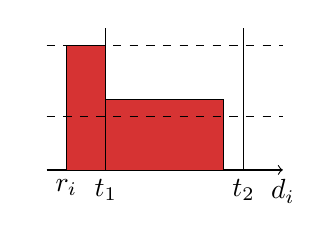
\begin{tikzpicture} [xscale=0.5,yscale=0.45]
      \node (O) at (0,0) {};
      \draw [->] (0,0) -- (6,0);
      \fill[red!80!black!80] (0.5,0) rectangle (1.5,3.5);
      \fill[red!80!black!80] (1.5,0) rectangle (4.5,2);
      \draw (0.5,0) node[below] {$r_i$};
      \draw (6,0) node[below] {$d_i$};
      \draw (1.5,0) node[below] {$t_1$} -- (1.5,4);
      \draw (5,0) node[below] {$t_2$} -- (5,4);
      \draw[dashed] (0,1.5) node[left] {$\bmin$} -- (6,1.5);
      \draw[dashed] (0,3.5) node[left] {$\bmax$} -- (6,3.5);
      \draw (0.5,0) -- (0.5,3.5) -- (1.5,3.5) -- (1.5,2) -- 
      (4.5,2) -- (4.5,0);
    \end{tikzpicture}
    &
      \onslide<2->{
      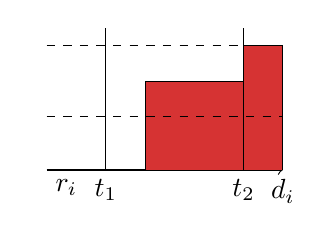
\begin{tikzpicture} [xscale=0.5,yscale=0.45]
        \node (O) at (0,0) {};
        \draw [->] (0,0) -- (6,0);
        \fill[red!80!black!80] (5,0) rectangle (6,3.5);
        \fill[red!80!black!80] (5,0) rectangle (2.5,2.5);
        \draw (0.5,0) node[below] {$r_i$};
        \draw (6,0) node[below] {$d_i$};
        \draw (1.5,0) node[below] {$t_1$} -- (1.5,4);
        \draw (5,0) node[below] {$t_2$} -- (5,4);
        \draw[dashed] (0,1.5) node[left] {$\bmin$} -- (6,1.5);
        \draw[dashed] (0,3.5) node[left] {$\bmax$} -- (6,3.5);
        \draw (6,0) -- (6,3.5) -- (5,3.5) -- (5,2.5) --
        (2.5,2.5) -- (2.5,0);
      \end{tikzpicture}

      ~~~~~~~~~~~~}
    \\
    \multicolumn{1}{c}{\small left-shifted} &
                                       \multicolumn{1}{c}{\only<2->{\small 
                                       right-shifted} }
  \end{tabular}
  
  \begin{overlayarea}{\textwidth}{3cm}
    \only<3-4>{
      \begin{tabular}{cc}
        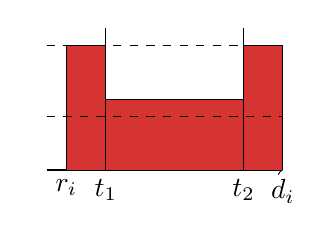
\begin{tikzpicture} [xscale=0.5,yscale=0.45]
          \node (O) at (0,0) {};
          \draw [->] (0,0) -- (6,0);
          \fill[red!80!black!80] (0.5,0) rectangle (1.5,3.5);
          \fill[red!80!black!80] (6,0) rectangle (5,3.5);
          \fill[red!80!black!80] (5,0) rectangle (1.5,2);
          \draw (0.5,0) node[below] {$r_i$};
          \draw (6,0) node[below] {$d_i$};
          \draw (1.5,0) node[below] {$t_1$} -- (1.5,4);
          \draw (5,0) node[below] {$t_2$} -- (5,4);
          \draw[dashed] (0,1.5) node[left] {$\bmin$} -- (6,1.5);
          \draw[dashed] (0,3.5) node[left] {$\bmax$} -- (6,3.5);
          \draw (0.5,0) -- (0.5,3.5) -- (1.5,3.5) -- (1.5,2) --
          (5,2) -- (5,3.5) -- (6,3.5) -- (6,0) ;
        \end{tikzpicture} 
        &
          \only<4>{
          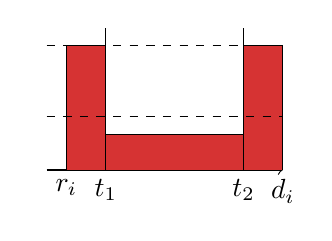
\begin{tikzpicture} [xscale=0.5,yscale=0.45]
                      \node (O) at (0,0) {};
          \draw [->] (0,0) -- (6,0);
          \fill[red!80!black!80] (0.5,0) rectangle (1.5,3.5);
          \fill[red!80!black!80] (6,0) rectangle (5,3.5);
          \fill[red!80!black!80] (5,0) rectangle (1.5,1);
          \draw (0.5,0) node[below] {$r_i$};
          \draw (6,0) node[below] {$d_i$};
          \draw (1.5,0) node[below] {$t_1$} -- (1.5,4);
          \draw (5,0) node[below] {$t_2$} -- (5,4);
          \draw[dashed] (0,1.5) node[left] {$\bmin$} -- (6,1.5);
          \draw[dashed] (0,3.5) node[left] {$\bmax$} -- (6,3.5);
          \draw (0.5,0) -- (0.5,3.5) -- (1.5,3.5) -- (1.5,1) --
          (5,1) -- (5,3.5) -- (6,3.5) -- (6,0) ;
          \end{tikzpicture}
          }
        \\
        \multicolumn{1}{c}{\small both-shifted 1} &
                                             \multicolumn{1}{c}{\only<4>{
                                             \small both-shifted 2}}
      \end{tabular}
    }
    \only<5-> {
      \begin{tabular}{cc}
        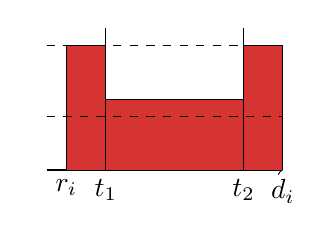
\begin{tikzpicture} [xscale=0.5,yscale=0.45]
          \node (O) at (0,0) {};
          \draw [->] (0,0) -- (6,0);
          \fill[red!80!black!80] (0.5,0) rectangle (1.5,3.5);
          \fill[red!80!black!80] (6,0) rectangle (5,3.5);
          \fill[red!80!black!80] (5,0) rectangle (1.5,2);
          \draw (0.5,0) node[below] {$r_i$};
          \draw (6,0) node[below] {$d_i$};
          \draw (1.5,0) node[below] {$t_1$} -- (1.5,4);
          \draw (5,0) node[below] {$t_2$} -- (5,4);
          \draw[dashed] (0,1.5) node[left] {$\bmin$} -- (6,1.5);
          \draw[dashed] (0,3.5) node[left] {$\bmax$} -- (6,3.5);
          \draw (0.5,0) -- (0.5,3.5) -- (1.5,3.5) -- (1.5,2) --
          (5,2) -- (5,3.5) -- (6,3.5) -- (6,0) ;
        \end{tikzpicture} 
        &
          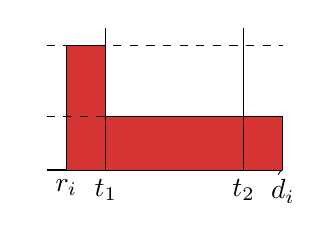
\begin{tikzpicture} [xscale=0.5,yscale=0.45]
            \node (O) at (0,0) {};
            \draw [->] (0,0) -- (6,0);
            \fill[red!80!black!80] (0.5,0) rectangle (1.5,3.5);
            \fill[red!80!black!80] (6,0) rectangle (1.5,1.5);
            \draw (0.5,0) node[below] {$r_i$};
            \draw (6,0) node[below] {$d_i$};
            \draw (1.5,0) node[below] {$t_1$} -- (1.5,4);
            \draw (5,0) node[below] {$t_2$} -- (5,4);
            \draw[dashed] (0,1.5) node[left] {$\bmin$} -- (6,1.5);
            \draw[dashed] (0,3.5) node[left] {$\bmax$} -- (6,3.5);
            \draw (0.5,0) -- (0.5,3.5) -- (1.5,3.5) -- (1.5,1.5) --
            (6,1.5)  -- (6,0) ;
          \end{tikzpicture}
        \\
        \multicolumn{1}{c}{\small both-shifted 1} &
                                             \multicolumn{1}{c}{
                                             \small both-shifted 2}
      \end{tabular}
    }
  \end{overlayarea}
\end{center}  
\end{frame}



\begin{frame}
  \frametitle{Energetic reasoning checker}
  We define the  slack function of interval $\inter$ as:
  \begin{gather}
    SL(t_1,t_2)={\color<2>{red}\text{ available space in
      }\inter}-{\color<2>{blue!50!}\text{ total mandatory }} \nonumber\\ 
        {\color<2>{blue!50!}\text{consumption in } \inter}\nonumber
  \end{gather}
  \begin{theorem}
    If there exists an interval on which the slack function is negative then there is no solution
  \end{theorem}
  \vfill
  \onslide<2>{
    \begin{center}
      \begin{tikzpicture}
        [transform shape,xscale=0.7,yscale=0.5]
        [inner sep=0pt]
        \node (O) at (0,0) {};
        \node[right of=O, node distance=6cm] (T) {};
        \node[right of=O, node distance=2cm] (t1) {};
        \node[right of=O, node distance=4cm] (t2) {};
        
        \draw[dashed] (0,4) node[left] {\Large$B$} -- (6,4);

        \draw[->] (O) -- (T);

        \draw[thick,red] (t1) -- (2,4.5);
        \draw[thick,red] (t2) -- (4,4.5);

        \draw[fill=blue!10!] (t1) node[above=2cm,left=0.6cm] {\color{blue!50!} \Large mandatory consumption} rectangle (4.5,4);
        \draw[pattern=north west lines, pattern color=red] (t1) rectangle (4,4) node[below=2cm,right=0.8cm] {\color{red} \Large available resource};
      \end{tikzpicture}
    \end{center}}
\end{frame}

\begin{frame}
  \frametitle{Relevant intervals}
  {\bf Question: } On which intervals $\inter$?\\
  \vfill
  $\rightarrow$ Analysis of the variation of the slack function\\
  \vfill
  \begin{block}{Slack function}
    \centering $SL(t_1,t_2)=B(t_2-t_1) - \sum_{i \in A} \bb$
  \end{block}
  \vspace{0.8cm}
  $\rightarrow$ Variation of $SL(t_1,t_2)$ depends on variation of 
  $\sum_{i \in A} \bb$
  \vfill 
\end{frame}


\subsubsection{Energetic reasoning filter}

\begin{frame}
  \frametitle{Time window adjustments}
  \vspace{0.4cm}
  \begin{center}
    \begin{tikzpicture}
  [yscale=0.5,xscale=0.9]
  \node[] (O) at (0,0) {};
  \node[label={[shift={(-0.4,-0.4)}]\small $b_i^{min}$}] (bmin) at (0,1) {};
  \node[label={[shift={(-0.4,-0.4)}]\small $b_i^{max}$}] (bmax) at (0,4) {};
  \node[label={[shift={(-0.4,-0.4)}]\small $B$}] (B) at (0,6) {};
  \node[label={[shift={(0,-0.8)}]\small $t_1$}] (t1) at (2.5,0) {}; 
  \node[label={[shift={(0,-0.8)}]\small $t_2$}] (t2) at (6,0) {};
  % \node[label={[shift={(0,-0.8)}]\small $d_i$}] (di) at (7,0) {};
  

  \onslide<5->{
    \draw[fill=gray!50!black!30] (4.25,1) --(6,1) -- (6,6) -- (2.5,6) --
    (2.5,1) --  (2.5,0)  -- (4.25,0) -- (4.25,1) -- cycle;
    \draw[pattern=north east lines, pattern color=blue!80!black!80] (4.25,0) rectangle (6,1);
    \draw[pattern=north east lines, pattern color=blue!80!black!80] (6,0) rectangle (7.5,4);
    \node[label={[shift={(0,-0.8)}]\small \color{red} $est_i$}] (ri) at
    (4.25,0) {}; 
    \draw(ri.south) -- (ri.center);
  } 
  \draw[->] (O.center) -- (8,0);
  \draw (O.south) -- (B.north);
  \draw (B.center) -- (8,6);
  \draw[dashed] (bmin.center) -- (8,1);
  \draw[dashed] (bmax.center) -- (8,4);
  
  % \draw(di.south) -- (di.center);
  \draw[thick] (t1.south) -- (2.5,6.1);
  \draw[thick] (t2.south) -- (6,6.1);
  
  % \onslide<1>{
  % \draw[fill=gray!50!black!30] (4.25,1) --(6,1) -- (6,6) -- (2.5,6) -- (2.5,1) --  cycle;
  % \draw[pattern=north west lines, pattern color=red!80!black!80] (6,0) rectangle (2.5,1);
  % \node[label={[shift={(0,-0.8)}]\small $est_i$}] (ri) at (1.5,0) {}; }

  \onslide<2>{
    \draw[fill=gray!50!black!30]  (6,6) rectangle (2.5,1)
    node[color=gray!50!black!80, midway,text width= 2cm]
    {\small $\sum_{i \neq j} \bb[j]$};
    \draw[pattern=north west lines, pattern
    color=red!80!black!80] (6,0) rectangle (2.5,1); 
    \node[label={[shift={(0,-0.8)}]\small $est_i$}] (ri) at (1.5,0) {}; 
    \draw(ri.south) -- (ri.center);}

\onslide<1-2>{
    \node[label={[shift={(0,-0.8)}]\small $est_i$}] (ri) at (1.5,0)
    {}; 
}

  \onslide<3-4>{
    \draw[fill=gray!50!black!30] (4.25,1) --(6,1) -- (6,6) -- (2.5,6) -- (2.5,1) --  cycle;
    \draw[pattern=north west lines, pattern
    color=red!80!black!80] (6,0) rectangle (2.5,1); 
    \node[label={[shift={(0,-0.8)}]\small $est_i$}] (ri) at (1.5,0){}; 
    \draw(ri.south) -- (ri.center);
    \draw[pattern=north east lines, pattern color=blue!80!black!80] (1.5,0) rectangle (2.5,4);}

  \onslide<3>{
    \draw[pattern=north east lines, pattern color=blue!80!black!80] (2.5,0) rectangle (6,3);
  }

  \onslide<4>{
    \draw[pattern=north east lines, pattern color=blue!80!black!80] (6,0) rectangle (7,4);
    \draw[pattern=north east lines, pattern color=blue!80!black!80] (2.5,0) rectangle (6,1.5);
  } 

\end{tikzpicture}

  \end{center}
  \vfill
  \begin{block}{Adjustments}
    if {\color<1-3>{red!80!black!80} available space for $i$}$<${\color<2-3>{blue!80!black} consumption of $i$ starting at $r_i$}  then
    \[\color<4>{blue!80!black}r_i \text{ can be adjusted}\]
  \end{block}
  \vfill
\end{frame}

\subsubsection{Other filtering algorithms}
\begin{frame}{Other filtering algorithms}

\end{frame}
\subsection{Mixed Integer Linear Program}

\begin{frame}{Justification of event-based model}

\end{frame}
\begin{frame}{Start/End model?}

\end{frame}


\begin{frame}
  \frametitle{An event-based formulation}
  {\small \it Adaptation of a model for the RCPSP {\color{gray!50!black!50} \it [Koné et al., 2011]}}
  \vfill
  \begin{block}{Variables}
    \begin{itemize}
    \item  $t_e$ represents the event (start or end time)
      \vspace{0.3cm}
    \item $z_{ie}=\left\{
        \begin{array}{ll}
          1 & \text{if $i$ is in process during $[t_{e},t_{e+1}]$}\\
          0 & \text{sinon}
        \end{array}
      \right.
      $
      \vspace{0.3cm}
    \item $B_{ie}$: resource quantity consumed by $i$ in $\inter[t_e][t_{e+1}]$
      \vspace{0.3cm}
    \item $W_{ie}$: energy brought to $i$ in $\inter[t_e][t_{e+1}]$   
    \end{itemize}
  \end{block}
\end{frame}
\subsection{Computational results}
\begin{frame}
  \frametitle{Computational results}
  \begin{block}{Instance generation}
    \begin{itemize}
    \item 5 instances 10, 60 tasks, 10 instances of 20, 25, 30 tasks. 
    \item random  $a_i$ and $c_i,\ \forall i \in A$, in ${[}1,10{]}$ and $W_i$ in ${[}0,f_i(W_i){]}$
    \end{itemize}
  \end{block}
  \begin{block}{Configuration}
    \begin{itemize}
    \item Intel Core i7-4770 processor with 4 cores and 8Go of RAM
    \item OS: 64-bit Ubuntu 12.04
    \item MILP resolution: CPLEX 12.6  
    \item BB : C++ and CPLEX at each leaf
    \item time limit: 7200 seconds
    \end{itemize}
  \end{block}
  

\end{frame}


\begin{frame}
  \frametitle{Computational results}
  \begin{figure}[!htb]
    \centering
    \includegraphics[width=0.9\linewidth]{figures/BB_time.png}
    \caption{Results of experiments for MILP model and hybrid branch-and-bound 
      for various parameters $\epsilon$ (CPU time in sec.)}
  \end{figure}

\end{frame}


\begin{frame}
  \frametitle{Computational results}
  \begin{figure}[!htb]
    \centering
    \includegraphics[width=0.9\linewidth]{figures/BB_solved.png}
    \caption{Percentage of solved instances for MILP model and hybrid 
      branch-and-bound (\% of solved instances)}
  \end{figure}
\vfill
\end{frame}

\section{General Conclusions and Perspectives}

\begin{frame}
  \frametitle{Conclusion}
  \vfill
  \begin{itemize}
  \item The general CECSP is a difficult problem
    \vfill
    \pause
  \item Description of properties allowing us to define solution
    methods:

      \vspace{0.2cm}
    \begin{description}["Hybrid" :]
      \pause
    \item[MILP : ]
      \begin{itemize}
      \item 3 models : Time-Indexed, Start/End, On/Off
      \item Improvement of the formulation: ER inequalities (TI),
        polyhedral study and valid inequalities (EB) 
      \end{itemize}
      
      \vspace{0.2cm}
      \pause
    \item[CP :] 
      \begin{itemize}
      \item TT, DR, TTDR
      \item ER : checker + filter + full caracterization of relevant
        interval
      \item TTFB: new checker (using LP!)
      \end{itemize}
      
      \vspace{0.2cm}
      \pause
    \item["Hybrid" :]
      \begin{itemize}
      \item Hybrid Branch-and-bound
      \item ER inequalities
      \item TTFB...
      \end{itemize}
    \end{description}
  \end{itemize}
\end{frame}

  \begin{frame}
    \frametitle{Perspectives}
    \vfill
    \begin{itemize}
    \item Improve MILP formulations
      \pause
      \begin{itemize}
      \item deduce inequalities from CP-reasoning
      \item Strengthening of event-based model
      \end{itemize}
      \vfill
      \pause
    \item Study of the discrete version of the problem
      \begin{itemize}
        \pause
      \item solutions are obtained faster  
      \item provide good approximation
      \end{itemize}
      \vfill
      \pause
    \item Consider more realistic power processing rate functions
      $f_i$
      \begin{itemize}
        \pause
      \item convex functions
      \item concave/convex functions
      \end{itemize}
      \vfill
      \pause
    \item Improve filtering algorithms
      \begin{itemize}
        \pause
      \item dedicated filtering algorithms
      \item improve ER : adaptation of $O(n^2 log n)$ algorithm
        {\small \it \color{gray!50!black!50} [Bonifas, 2016], [Tesch,
          2016]}  
      \end{itemize}
    \end{itemize}
    \vfill
  \end{frame}

  \begin{frame}{Energy/Resource model}
    \vfill
    \begin{block}{On/Off model}
      {\footnotesize
        \begin{align*}
          &\sum_{i\in A} B_{ie} \le B(t_{e+1}-t_e)
          &\forall e & \tag{\it \scriptsize
                                                    cumulative}\\
        &  B_{ie} \ge \bmin(t_{e+1}-t_e) -
M{\color{blue!80!black!80}(1-z_{ie})} & \forall e;\ \forall i & \tag{\it \scriptsize
                                       min consump.}\\ 
          &B_{ie} \le \bmax(t_{e+1}-t_e) &\forall e ;\ \forall i& \tag{\it \scriptsize
                                       max consump.}\\
          &{\color{red!80!black!80}z_{ie}}M\ge B_{ie} &\forall
e;\ \forall i  &\tag{\it \scriptsize
                 no consump.}\\
& & &\\
          &W_{ie} \le a_iB_{ie}+c_i(t_{e+1}-t_{e}) &
\forall e;\ \forall i \in A& \tag{\it
                                                          \scriptsize conv res. / nrj}\\
         & W_{ie} \le
W_i{\color{red!80!black!80}z_{ie}} &\forall e ;\ \forall i& \tag{\it
                                                             \scriptsize
                                                             no 
                                                             nrj}\\
          &\sum_{e \in 
{\cal E}\setminus \{2n\}} W_{ie} = W_i &\forall i &\tag{\it
\scriptsize required nrj}
        \end{align*}
      }
    \end{block}
    \vfill
  \end{frame}

\addtocounter{framenumber}{-1}
  
  \begin{frame}{Event-based model}
  \vfill 
  {\bf On/Off Model}
  {\footnotesize
    \begin{eqnarray*}
      \textcolor<1>{blue!80!black!80}{t_e \le t_{e+1} }&
                                                         \textcolor<1>{blue!80!black!80}{ \forall e}\\[2mm]
      \pause
      \textcolor<2>{blue!80!black!80}{r_iz_{ie}\le t_e
      } & \textcolor<2>{blue!80!black!80}{\forall e, i
          }\\[2mm] 
      \textcolor<2>{blue!80!black!80}{t_e \le
      lst_i(z_{ie}-z_{ie-1})+(1-(z_{ie}-z_{ie-1}))D_{max} }&
                                                             \textcolor<2>{blue!80!black!80}{ \forall e,i}\\[2mm]
      \pause
      \textcolor<3>{blue!80!black!80}{ 
      eet_i(z_{ie-1}-z_{ie})\le t_e} & \textcolor<3>{blue!80!black!80}{
                                       \forall e, i }\\[2mm]
      \textcolor<3>{blue!80!black!80}{t_e \le
      d_i(z_{ie-1}-z_{ie})+(1-(z_{ie-1}-z_{ie}))D_{max}}&
                                                          \textcolor<3>{blue!80!black!80}{\forall e, i }\\[2mm]
      \pause
      \textcolor<4>{blue!80!black!80}{ \sum_{e \in {\cal E}}
      z_{ie} \ge 1}& \textcolor<4>{blue!80!black!80}{\forall i
                     } \\[2mm]
      \textcolor<4>{blue!80!black!80}{\sum_{e'=1}^{e}
      z_{ie'} \le e(1-(z_{ie}-z_{ie-1})) }& \textcolor<4>{blue!80!black!80}{
                                            \forall e,i}\\[2mm]
      \textcolor<4>{blue!80!black!80}{\sum_{e'=e}^{2n}
      z_{ie'} \le (2n-e)(1+(z_{ie}-z_{ie-1})) }&
                                                 \textcolor<4>{blue!80!black!80}{\forall e,i}
    \end{eqnarray*}}
  \vfill
\end{frame}
\addtocounter{framenumber}{-1}
  



\pgfplotstableread[row sep=\\,col sep=&]{
  tasks & Default & Int. &  Preem. & I+P \\
  30    & 34.8 & 30.3& 30.3& 33.1\\
}\mydat
\begin{frame}
  \frametitle{Time comparison for the RCPSP}
  \begin{itemize}
  \item Instances of {\color{gray!50!black!70} \it [Koné et al., 2011]}
  \item 480 instances of 30 tasks
  \end{itemize}

  \vspace{0.3cm}
  \begin{center}
    \begin{tikzpicture}
      \begin{axis}[ enlarge x limits=0.25,
        ybar,
        bar width=.8cm,  
        legend style={at={(0.5,1)},
          anchor=north,legend columns=-1},
        width=0.8\textwidth,
        height=.55\textwidth,
        symbolic x coords={30},
        xtick=data,
        ymin=0,ymax=50,
        ylabel={\small $time (s)$},
        xlabel={\small $\#tasks$}]
        \addplot table[x=tasks,y=Default]{\mydat};
        \addplot table[x=tasks,y=Int.]{\mydat};
        \addplot table[x=tasks,y=Preem.]{\mydat};
        \addplot table[x=tasks,y=I+P]{\mydat};
        \legend{Default ,Int. , Time , Preem. ,I+T+P}
      \end{axis}
    \end{tikzpicture}
  \end{center}
\end{frame}

\addtocounter{framenumber}{-1}
\end{document}






